\documentclass[numbers,sort&compress]{IntechOpen-Book}%%OPTIONS are numbers, authoryear, sort&compress,sectref

\graphicspath{{Artworks/}}

\usepackage{amsmath,amssymb}
\usepackage{runic}

% wasysym redefinitions
\newcommand*{\wasyfamily}{\fontencoding{U}\fontfamily{wasy}\selectfont}
\newcommand*{\astrosun}{{\odot}}
\newcommand*{\mercury}{{\text{\wasyfamily\char39}}}
\newcommand*{\venus}{{\text{\wasyfamily\char25}}}
\newcommand*{\earth}{{\oplus}}
\newcommand*{\mars}{{\text{\wasyfamily\char26}}}
\newcommand*{\jupiter}{{\text{\wasyfamily\char88}}}
\newcommand*{\saturn}{{\text{\wasyfamily\char89}}}
\newcommand*{\uranus}{{\text{\wasyfamily\char90}}}
\newcommand*{\neptune}{{\text{\wasyfamily\char91}}}
\newcommand*{\pluto}{{\text{\wasyfamily\char92}}}

% mathabx definitions
\newcommand*{\mathabxbfamily}{\fontencoding{U}\fontfamily{mathb}\selectfont}
\DeclareFontFamily{U}{mathb}{\hyphenchar\font45}
\DeclareFontShape{U}{mathb}{m}{n}{
      <5> <6> <7> <8> <9> <10> gen * mathb
      <10.95> mathb10 <12> <14.4> <17.28> <20.74> <24.88> mathb12
      }{}
\newcommand*{\Sun}{{\text{\mathabxbfamily\char"40}}}
\newcommand*{\Mercury}{{\text{\mathabxbfamily\char"41}}}
\newcommand*{\Venus}{{\text{\mathabxbfamily\char"42}}}
\newcommand*{\Earth}{{\text{\mathabxbfamily\char"43}}}
\newcommand*{\Mars}{{\text{\mathabxbfamily\char"44}}}
\newcommand*{\Jupiter}{{\text{\mathabxbfamily\char"45}}}
\newcommand*{\Saturn}{{\text{\mathabxbfamily\char"46}}}
\newcommand*{\Uranus}{{\text{\mathabxbfamily\char"47}}}
\newcommand*{\Neptune}{{\text{\mathabxbfamily\char"48}}}
\newcommand*{\Pluto}{{\text{\mathabxbfamily\char"49}}}

\newcommand*{\astrosymbolsA}{\astrosun\mercury\venus\earth\mars\jupiter\saturn\uranus\neptune\pluto}

\newcommand*{\astrosymbolsB}{\Sun\Mercury\Venus\Earth\Mars\Jupiter\Saturn\Uranus\Neptune\Pluto}


\renewcommand\refname{\textfut{REFERENCES}}

\begin{document}

\Mainmatter

\begin{frontmatter}

\chapter{\textfut{INTRODUCTION CHAPTER - ASTRONOMY}}
% Enter author names EXACTLY as you would like them to appear in the final manuscript; only use pattern: first name, last name. Do NOT use pattern: last name, first name. Patronyms fall into the first name category.
\author{\textfut{YANN-HENRI CHEMIN}}
%\author{Author 2}
%\author{Author 3}

\makechaptertitle

\chaptermark{\textfut{INTRODUCTION CHAPTER - ASTRONOMY}}

\end{frontmatter}

\section{\textfut{INTRODUCTION}}
%This is intro for bibitem 
\textfut{THE OBSERVATION OF THE SUN, THE SOLAR SYSTEM, AND THE VAST REGIONS LAYING OUTSIDE, ARE COMMONLY CALLED ASTRONOMY}. 

\textfut{IN THE WHOLE RANGE OF OBSERVATIONS OF OUR NEIGHBOURHOOD} (\textfut{FIGURE }\ref{intro:fig01}), \textfut{ WE STUDY THE SUN, THE MOON, THE ROCKY PLANETS AND THE GAS GIANTS. IN THE LAST DECADES, THE SPACE PROBES SENT AROUND THE SOLAR SYSTEM HAVE ENHANCED OUR EXPLORATION CAPACITY, THAT IS TO GO FROM HAZY PHOTOGRAPHS TO HIGH RESOLUTION MAPPING OF MOST OF OUR PLANETARY BODIES, EVEN OF THEIR MOONS. ADDITIONALLY, DWARF PLANETS (CERES, VESTA) AND ASTEROIDS HAVE BEEN VISITED, AND MAPPED. THIS, IN ITSELF, IS A UNIQUE CIVILISATIONAL ACHIEVEMENT, IN TERMS OF EXPLORATION.}

\textfut{IN BETWEEN MARS AND JUPITER, THE ASTEROID BELT IS FOUND. FURTHER AND MOSTLY AFTER NEPTUNE ORBIT IS THE KUIPER BELT. EVENTUALLY, THE VERY POSSIBLE OORT CLOUD, A RESERVOIR OF VISITING COMETS, VASTLY BEYOND THE ORBIT OF }(90377) \textfut{SEDNA} (\textfut{FIGURE} \ref{intro:fig01}). 

\textfut{OUR SOLAR SYSTEM IS LOCATED IN BETWEEN TWO ARMS OF A SPIRAL GALAXY, WITHIN A WHAT IS OFTEN CALLED A ``FINGER'' NAMED THE ORION SPUR} ( \textfut{FIGURE} \ref{intro:fig02}). \textfut{THE CENTER OF OUR GALAXY, THE MILKY WAY, IS THE SEAT OF A SUPER MASSIVE BLACK HOLE ``SMBH'' CALLED SAGITTARIUS A*} \cite{intro:bib01}. 

\textfut{OUR GALAXY IS LOCATED ON A FRINGE OF WHAT COULD BE CALLED ``MYCELIUM'' FILAMENTS. IN OTHER WORDS, DETECTABLE MATTER AT COSMOLOGICAL LEVEL, TENDS TO AGGLOMERATE IN THREADS, INTERCONNECTED BY GROUPS OF LARGER MATERIAL AGGREGATIONS, NOT UNLIKE THE SPREAD OF FUNGAL MYCELIUM IN EARTH'S SOIL, PUNCTUATED BY THE PRESENCE OF ``NODES'', FROM WHICH MYCELIUM FILAMENTS EXTEND. OF PARTICULAR IMPORTANCE TO OUR GALAXY ``SUBURB'' IS A LARGE AREA VOID OF MATTER} (\textfut{FIGURE} \ref{INTRO:FIG03})\textfut{. THE ``LOCAL VOID'' HAS BEEN MAPPED SYNTHETICALLY WITH GREAT RESOLUTION RECENTLY.} \cite{intro:bib04}

\textfut{THE OVERALL OBSERVABLE UNIVERSE IS A SPHERE, CENTERED ON THE LOCATION OF THE ONE OBSERVING. FOR US, IT IS PLANET EARTH. WHEN MAPPED, THIS SPHERE, SO FAR, EXTENDS OUTWARDS IN A RADIUS OF 46.5 BILLION LIGHT-YEARS (440 YM), AS A COMOVING DISTANCE. THE SLOAN DIGITAL SKY SURVEY (SDSS), MAPPING OF THE OBSERVABLE UNIVERSE} \cite{intro:bib05},\textfut{ WAS DONE NOT BY DIRECT DISTANCE, BUT IN SIGNED VELOCITY FROM THE OBSERVATION POINT, DEDUCTING MOSTLY FROM THE RED-SHIFTING OF THE OBSERVATIONS. THE FASTEST THE POSITIVE RED-SHIFTING VELOCITY, THE FURTHER AWAY THE COLOCATION TO THE OBSERVER.}

%For the layout editors: Maybe these could go in a 2x2 frame on a separate page?
\begin{figure}[!b]
 \begin{minipage}[b]{0.5\linewidth}
    \centering
	\FIG{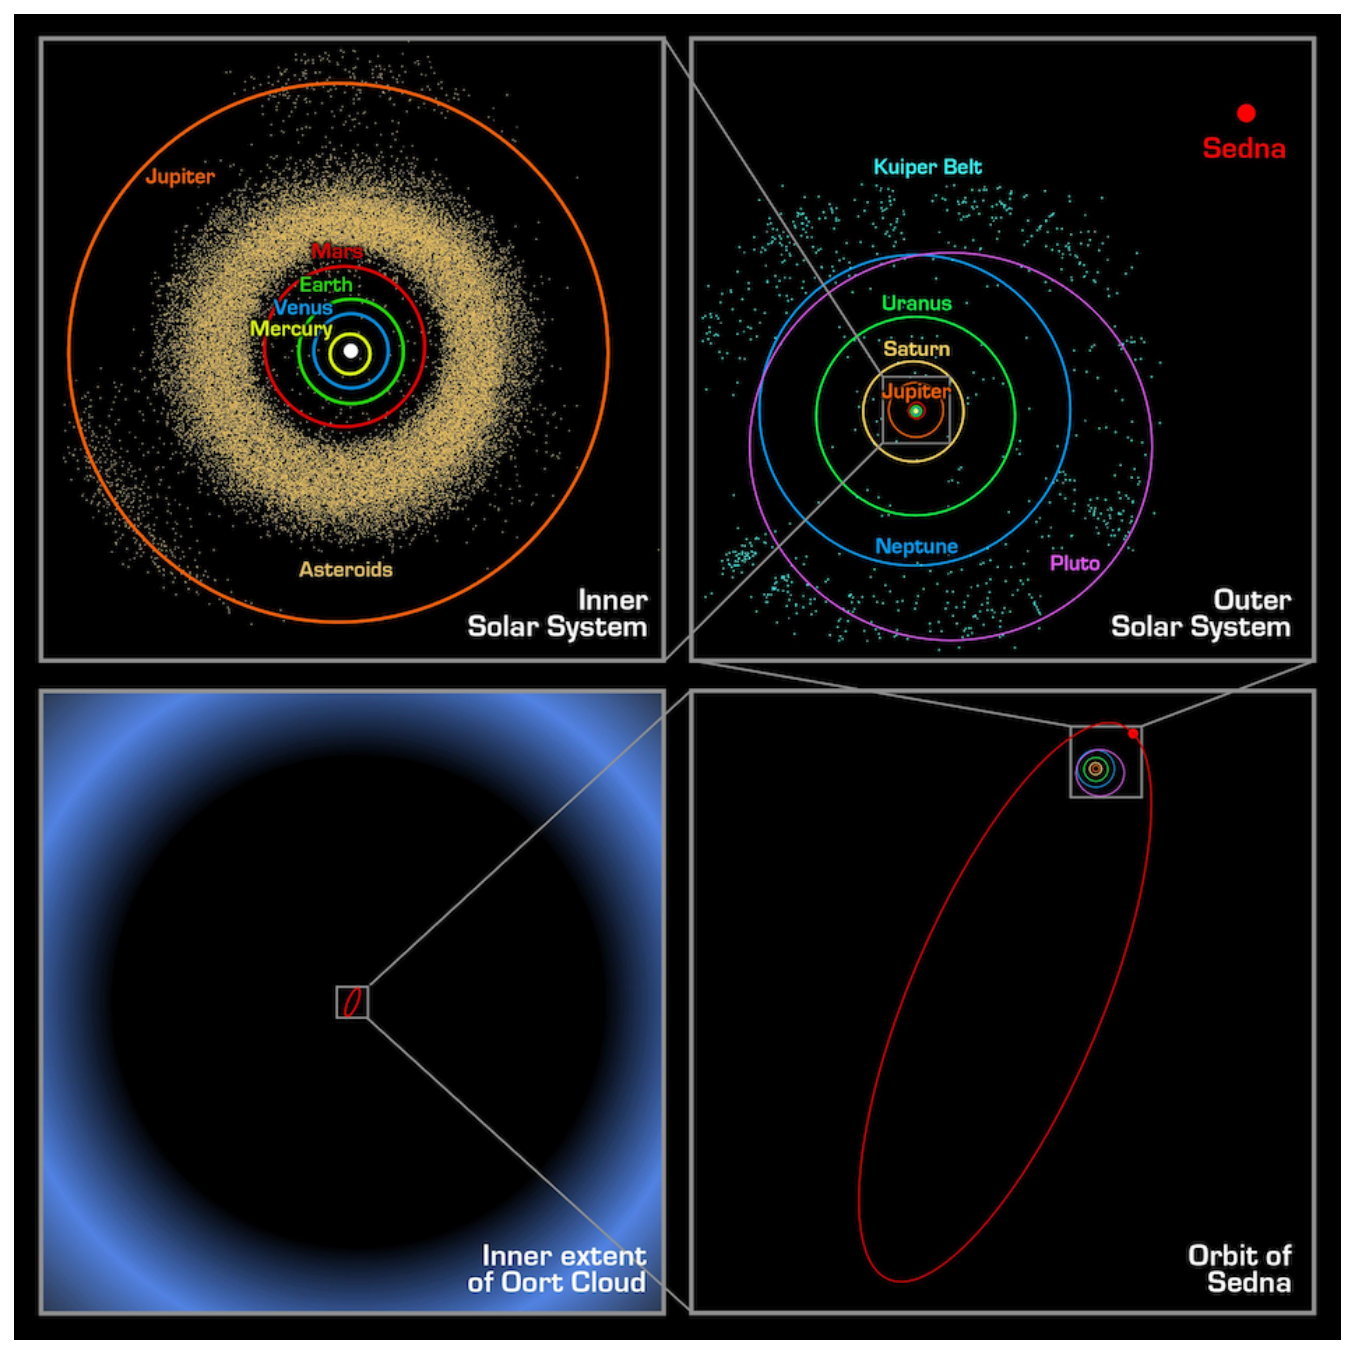
\includegraphics[width=\linewidth]{solarsystem_2208_12364}}
	{\caption{\textfut{EXTRACTED FROM} \cite{intro:bib02} \textfut{THIS IS THE SOLAR SYSTEM. UPPER LEFT IS DEFINED BY JUPITER ORBIT, UPPER RIGHT REACHES PLUTO'S ORBIT, THE KUIPER BELT AND THE PERIGEE OF} (90377) \textfut{SEDNA. BOTTOM RIGHT IS THE ORBIT OF} (90377) \textfut{SEDNA, WHICH IS BARELY SEEN IN BOTTOM LEFT ALONGSIDE THE INNER OORT CLOUD, WHAT IS THOUGHT TO BE THE SOURCE OF COMETS. IMAGE CREDIT: NASA/CALTECH}.\label{intro:fig01}}}
    \vspace{0ex}
\end{minipage}
 \begin{minipage}[b]{0.5\linewidth}
    \centering
	\FIG{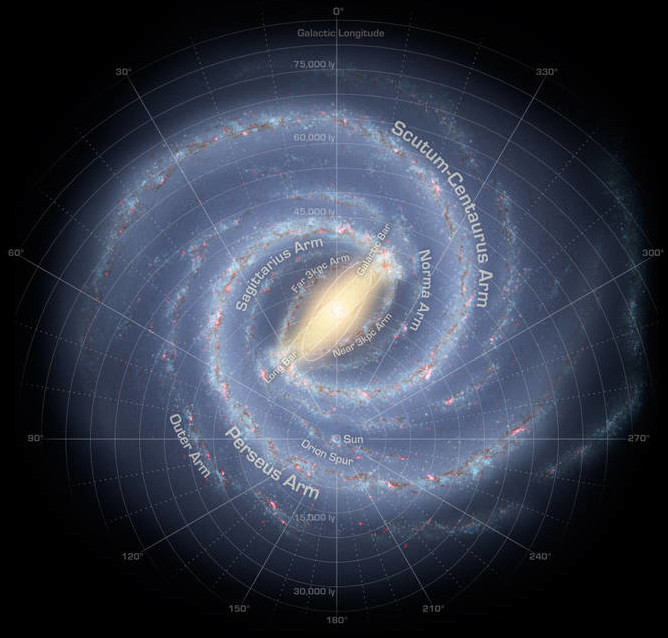
\includegraphics[width=\linewidth]{main_milkyway_full}}
	{\caption{\textfut{EXTRACTED FROM} \cite{intro:bib03} \textfut{IMAGE CREDIT: NASA/ADLER/U. CHICAGO/WESLEYAN/JPL-CALTECH.}\label{intro:fig02}}}
    \vspace{9.8ex}
\end{minipage}
 \begin{minipage}[b]{0.5\linewidth}
    \centering
	\FIG{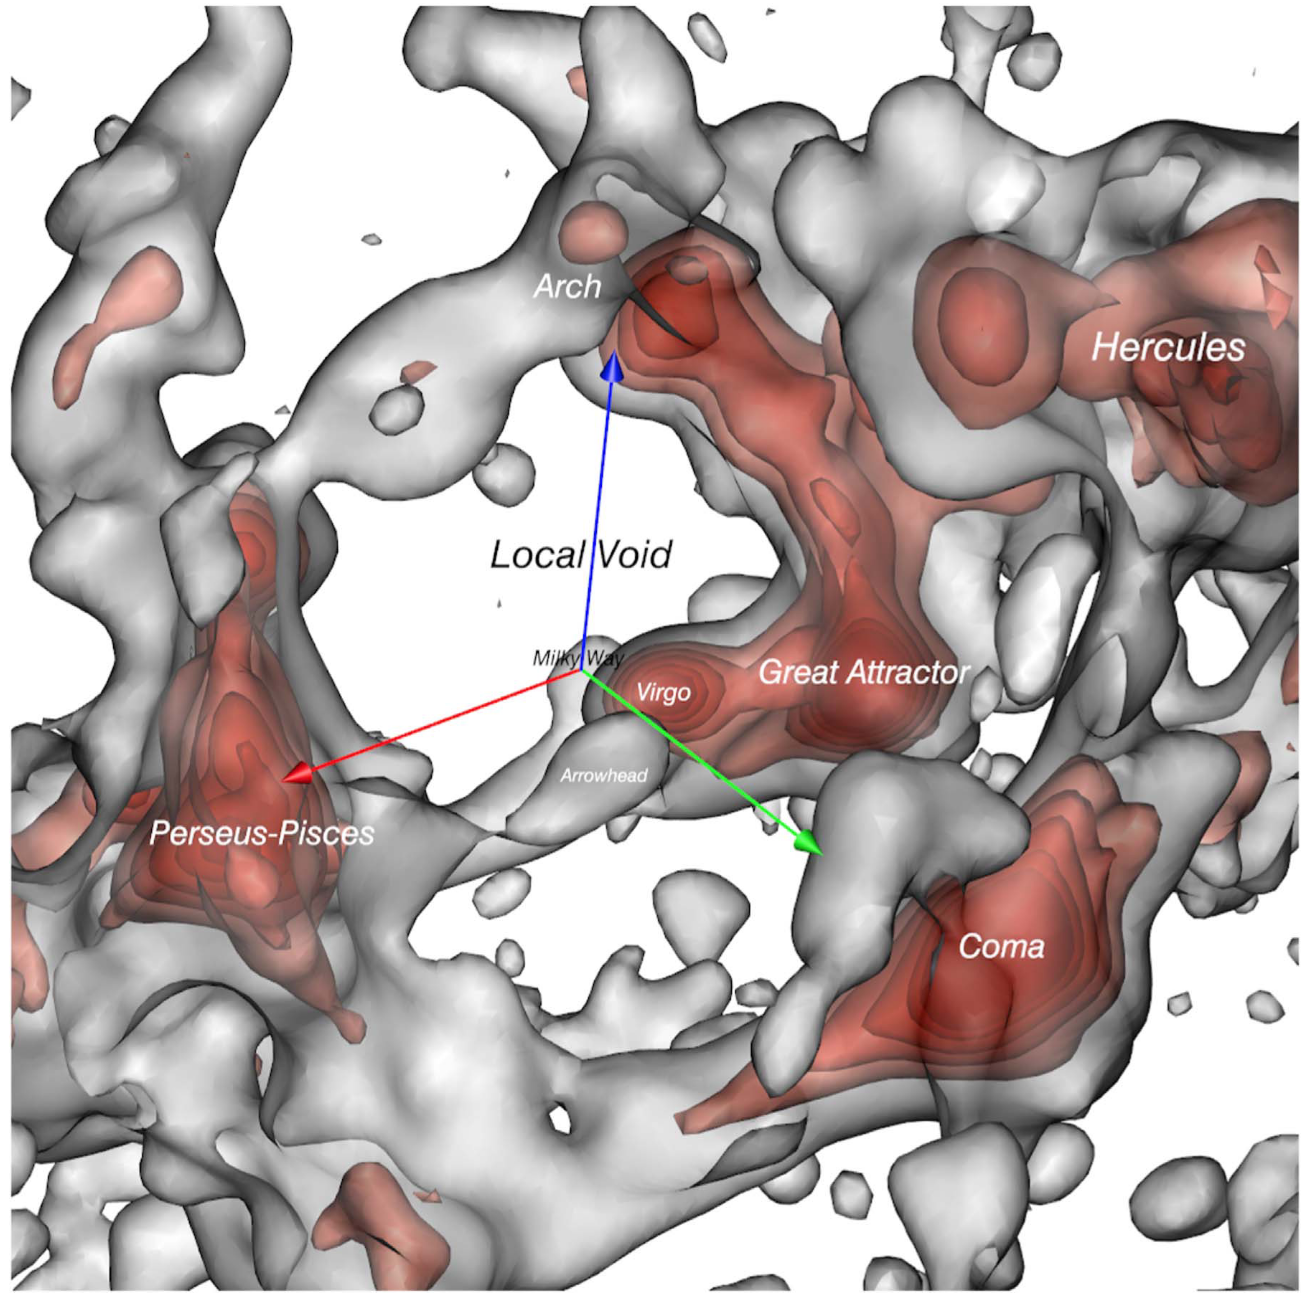
\includegraphics[width=\linewidth]{LocalVoid_Tully_2019_ApJ_880_24}}
	{\caption{\textfut{EXTRACTED FROM} \cite{intro:bib04} \textfut{THE ``LOCAL VOID'', VISUALIZATION CENTERED ON OUR GALAXY, THE MILKY WAY.} \label{intro:fig03}}}
    \vspace{8ex}
\end{minipage}
 \begin{minipage}[b]{0.5\linewidth}
    \centering
	\FIG{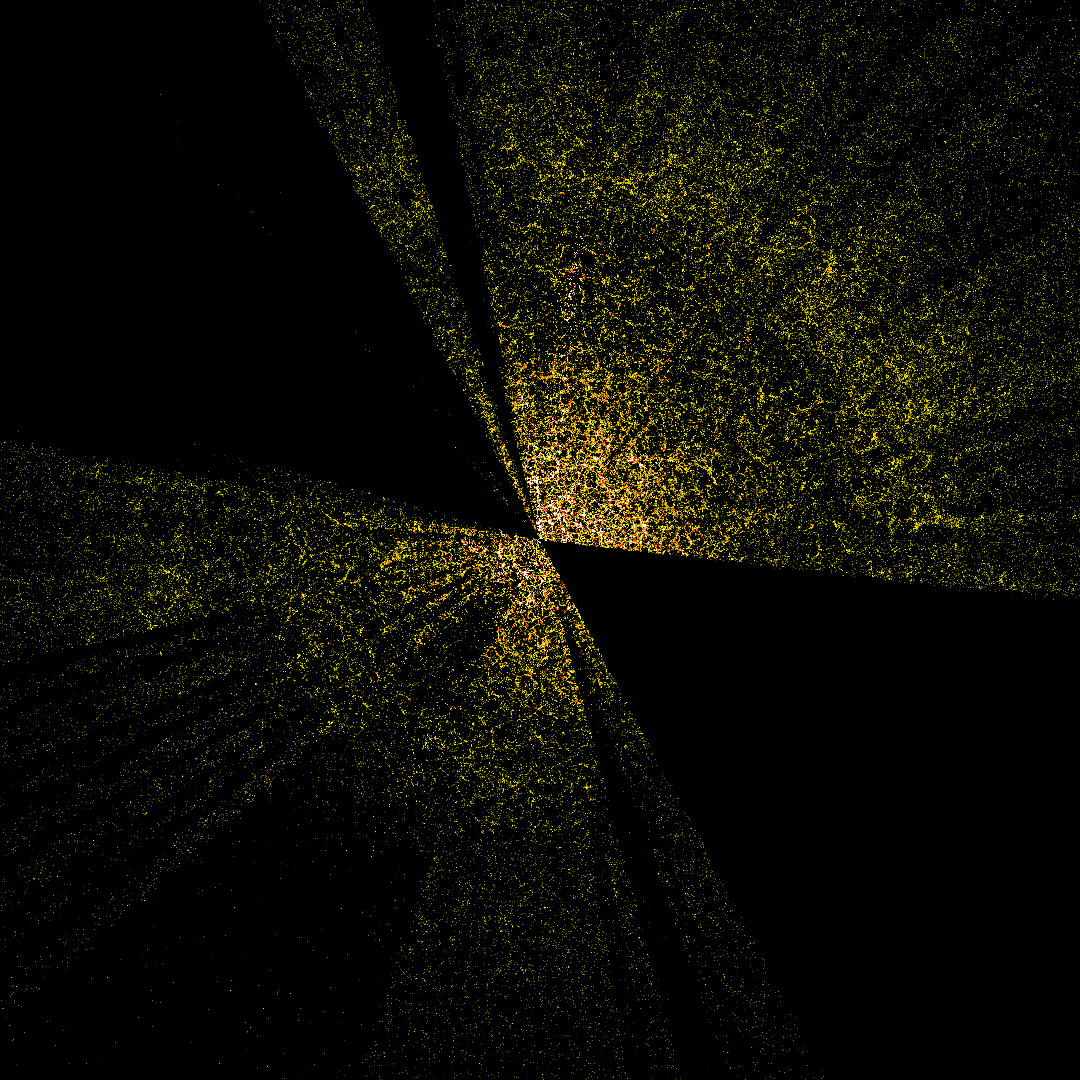
\includegraphics[width=\linewidth]{DESI_zmax1}}
	{\caption{\textfut{EXTRACTED FROM} \cite{intro:bib06} \textfut{SCANNING FROM THE DARK ENERGY SPECTROSCOPIC INSTRUMENT ``DESI'', FROM THE CENTER, EARTH, TOWARDS THE FURTHER SEEN SO FAR, ABOUT ONE BILLION OF YEARS AFTER THE BIG BANG.} \label{intro:fig04}}}
    \vspace{4.3ex}
  \end{minipage}
\end{figure}


\section{\textfut{OBSERVING THE SUN, AND THE STARS}}
%This is ch01 for bibitem

\textfut{THE CLOSEST OF THE STARS, THE SUN, IS A G-IV, MAIN-SEQUENCE STAR, AND IS LOCATED IN THE CENTER OF THE HERTZSPRUNG-RUSSELL ``HR'' DIAGRAM} \cite{ch01:bib01} \textfut{CLASSIFICATION} (\textfut{FIGURE} \ref{ch01:fig01}). \textfut{ITS NEXT EVOLUTIONS WOULD BE TO LEAVE THE MAIN SEQUENCE, THAT IS THE OBLIQUE LINE CROSSING FIGURE} \ref{ch01:fig01} \textfut{TOWARDS THE UPPER RIGHT. IT IS THEN GOING TO INFLATE AND SHIFT TO BECOME EVENTUALLY A RED GIANT, MOVING FURTHER UP IN THE UPPER RIGHT ARM OF THE HR DIAGRAM. ONCE REACH MAXIMUM INFLATION, A CASCADE OF GRAVITATIONAL COLLAPSES WILL HAPPPEN, EJECTING MATERIAL BY MAJOR EXPLOSIONS. GRAVITY WILL COMPACT THE REMAINING INTO A WHITE DWARF, A NEUTRON STAR, IN THE MIDST OF ITS EJECTA, WITNESSED AS A ``SUPER''NOVA REMNANT, A NEBULA.  THE TRANSITION FROM THE SUPER-GIANT, THE (SUPER)NOVA REDUCING INTO THE REMAINING WHITE DWARF, WILL TAKE THE STAR RAPIDLY ACROSS THE HR DIAGRAM, FROM THE UPPER RIGHT, TO THE MID-UPPER LEFT, AND CROSSING DOWN IN THE VISIBLE ARC IN THE BOTTOM LEFT SIDE OF FIGURE} \ref{ch01:fig01}. 

\textfut{THE CENTRAL PART OF THE SUN IS COMPOSED OF A CORE (A FOURTH OF ITS RADIUS) WHERE THERMONUCLEAR REACTIONS GENERATE ENERGY. IT HAS AN AVERAGE DENSITY TEN TIMES THAT OF LEAD, AND A TEMPERATURE OF} 15 10$^6$ \textfut{K. THE RADIATIVE ZONE OF THE SUN IS ABOUT ONE THIRD OF THE SUN'S RADIUS. BOTH TRANSFER ENERGY BY RADIATIVE FORCES OF PHOTONS. THE PATHWAYS UNDERGO A RANDOM WALK AND ACT AS AN APPARENT SOLID-BODY} \cite{ch01:bib02}. 

\textfut{THE PHOTOSPHERE IS 300-500 KM DEEP, THE LIGHT IS EMITTED FROM THERE, BEFORE THE PLASMA BECOMES OPAQUE. THIS IS ALSO THE LAYER THAT DEFINES THE EFFECTIVE TEMPERATURE OF THE SUN, ABOUT} 5.8 10$^3$ \textfut{K, PLASMA CONVECTION IS VISIBLE THERE UNDER THE FORM OF GRANULES OF SIZES MEASURED IN MM} (10$^3$ \textfut{M}).

\begin{figure}[!b]
 \begin{minipage}[b]{0.5\linewidth}
    \centering
	\FIG{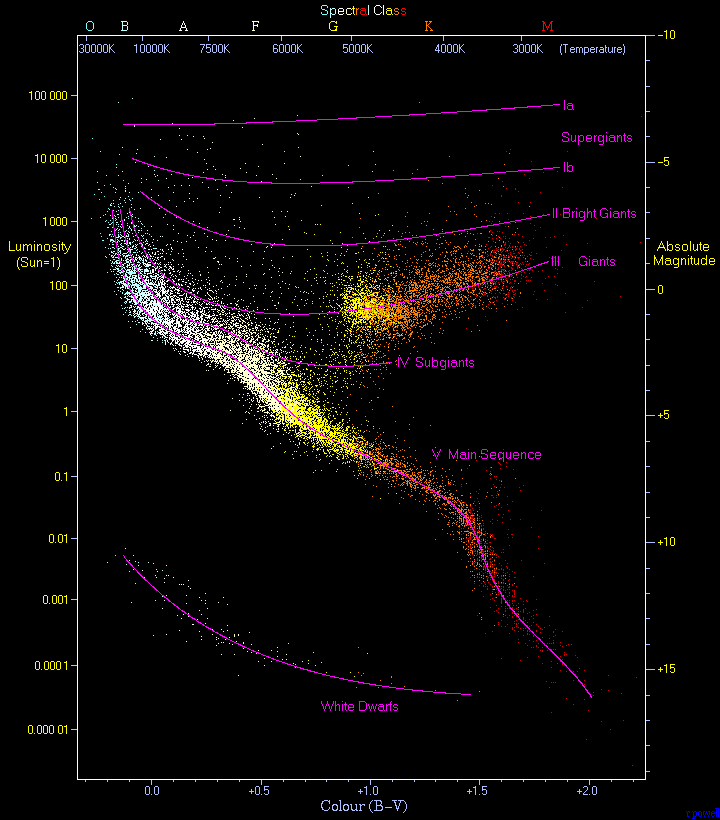
\includegraphics[width=\linewidth]{HRDiagram}}
	{\caption{\textfut{HR DIAGRAM, CLASSIFICATION OF STARS EVOLUTION. IMAGE CREDITS: WIKIMEDIA.} \label{ch01:fig01}}}
% source: https://upload.wikimedia.org/wikipedia/commons/6/6b/HRDiagram.png
    \vspace{4.3ex}
\end{minipage}
 \begin{minipage}[b]{0.5\linewidth}
    \centering
	\FIG{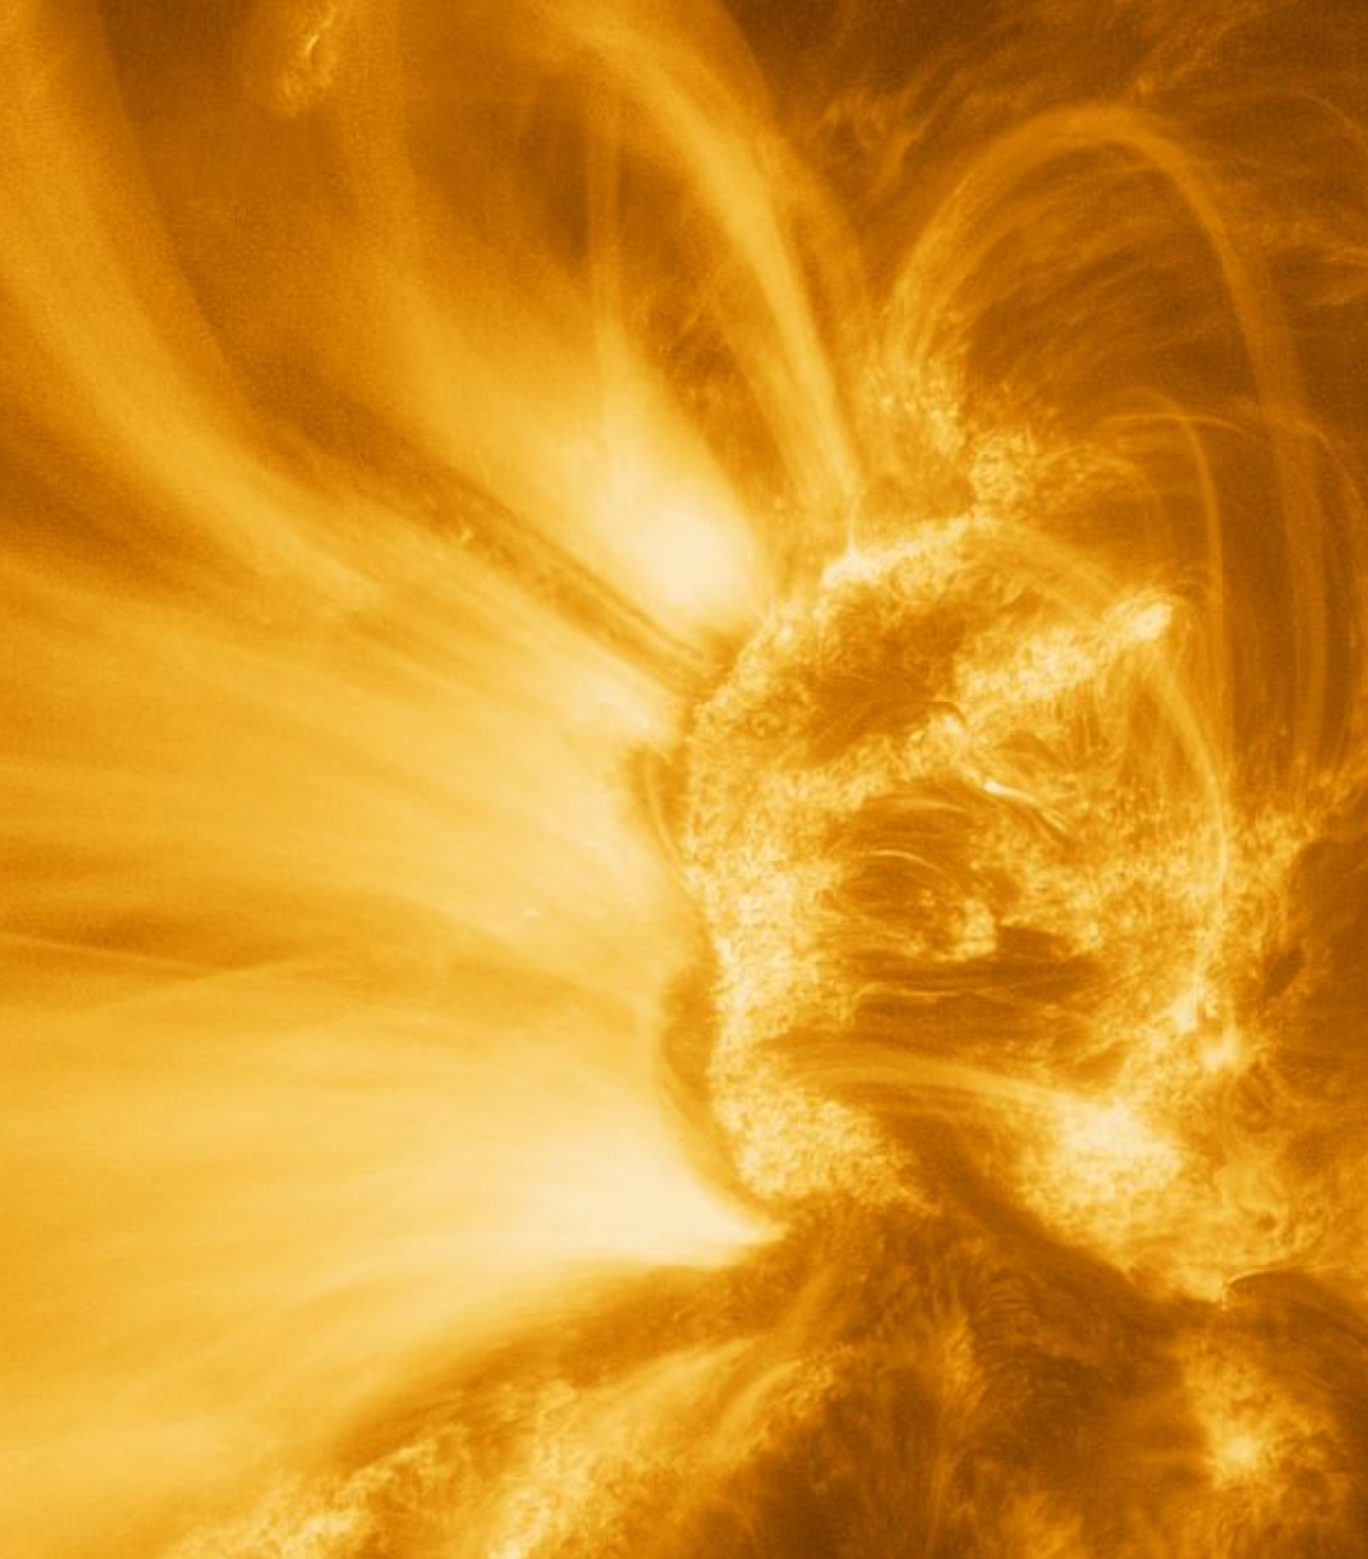
\includegraphics[width=\linewidth]{sunorbitersnap_small}}
	{\caption{\textfut{HIGH RESOLUTION IMAGE OF THE SUN FROM SOLAR ORBITER, SHOWING MAGNETICALLY BOUND PLASMA. CREDIT: ESA \& NASA/SOLAR ORBITER/EUI TEAM; DATA PROCESSING: E. KRAAIKAMP}. \cite{ch01:bib04}
\label{ch01:fig02}}}
    \vspace{0ex}
\end{minipage}
 \begin{minipage}[b]{0.5\linewidth}
    \centering
	\FIG{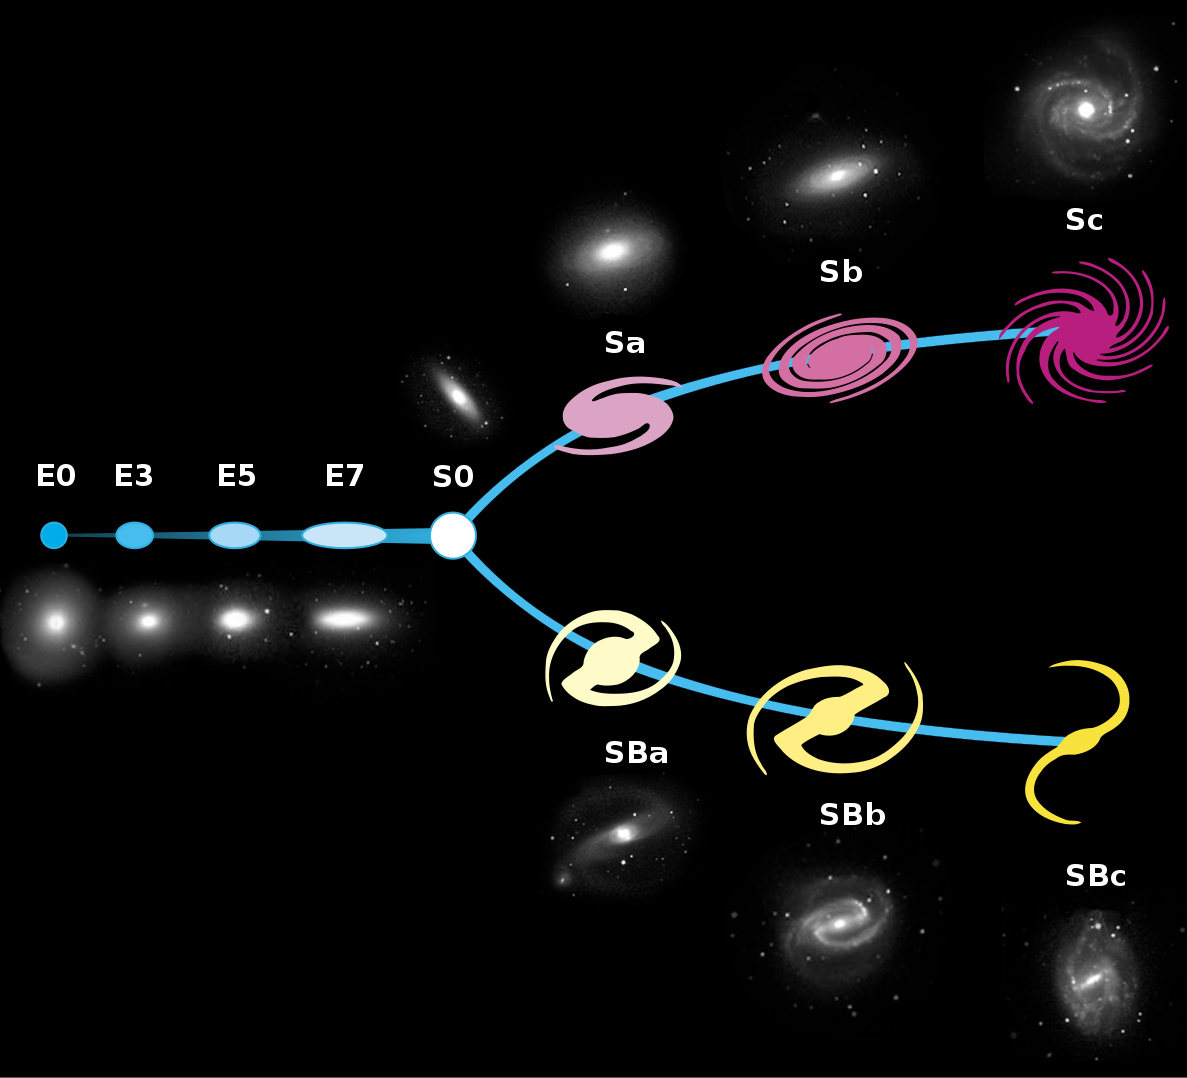
\includegraphics[width=\linewidth]{Hubble_Tuning_Fork_diagram}}
	{\caption{\textfut{HUBBLE CLASSIFICATION OF GALAXIES EVOLUTION, THE {HUBBLE SEQUENCE}. COURTESY: WIKIPEDIA.}
\label{ch02:fig01}}}
%Source: https://en.wikipedia.org/wiki/Hubble_sequence#/media/File:Hubble_Tuning_Fork_diagram.svg
    \vspace{5.5ex}
\end{minipage}
 \begin{minipage}[b]{0.5\linewidth}
    \centering
	\FIG{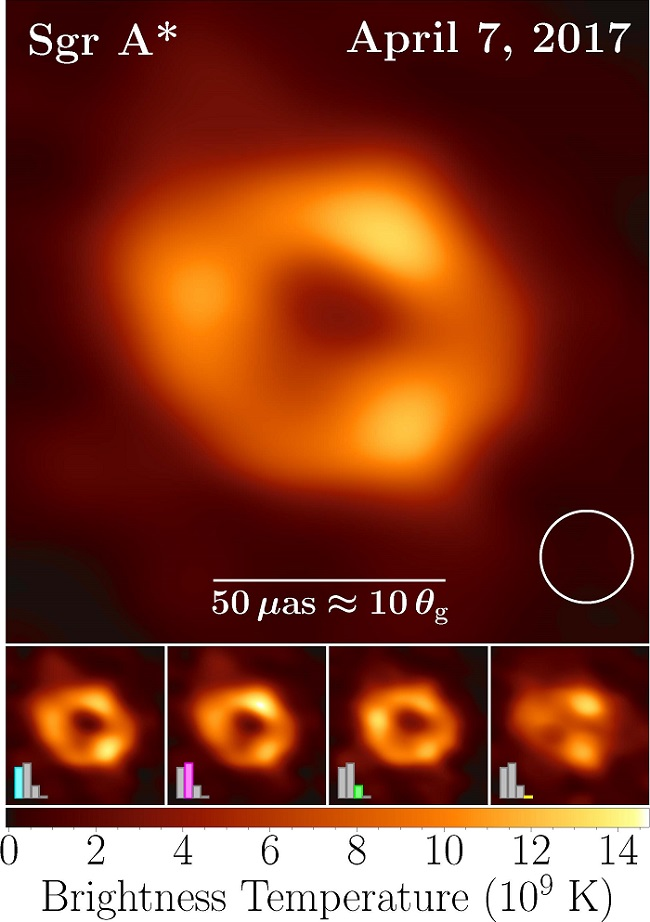
\includegraphics[width=\linewidth]{First_SGR_A_results}}
	{\caption{\textfut{EVENT HORIZON OF THE SMBH SGR A* AT THE CENTER OF THE MILKY WAY}\cite{ch02:bib03}
\label{ch02:fig02}}}
%Source: 
    \vspace{0ex}
  \end{minipage}
\end{figure}


\textfut{THE SUN'S ``ATMOSPHERE''} ( \textfut{STARTING FROM FIGURE} \ref{ch01:fig02}) \textfut{IS COMPOSED OF THE CHROMOSPHERE AND THE CORONA (IN THAT ORDER). THE CHROMOSPHERE IS 2000 KM DEEP AND IS THE SUN'S ECLIPSE ``RED RING OF FIRE''. IT HAS A STEEP DROP IN MATERIAL DENSITY, AND A AN INITIAL TEMPERATURE DROP FROM} 5.8 10$^3$ \textfut{K TO} 3.5 10$^3$ \textfut{K TO EVENTUALLY REACH} 35 10$^3$ \textfut{K}.

\textfut{THE CORONA IS A VERY LARGE VOLUME ABOVE THE CHROMOSPHERE, VASTLY WARMER TOO, MADE OF IONIZED PLASMA OF ABOUT} 1 106\textfut{K, WITH A MAJORITY OF EMISSION COMING FROM FE-XI}V\textfut{ AND FE-X. IT IS THE ORIGIN OF THE SOLAR WINDS. SOME AREAS WITH OPEN MAGNETIC FIELDS, YIELD FASTER SOLAR WINDS} (\textfut{ABOUT} 0.7 10$^6$ \textfut{M/S}). 

\textfut{WE REMOTELY SENSE THE SUN} (\textfut{SOLAR ORBITER IMAGERY IN FIGURE} \ref{ch01:fig02}), \textfut{BY ANALYSING ELECTROMAGNETIC SPECTRA EMITTED FROM ITS ACTIVITY. THERMODYNAMICS, HYDRODYNAMICS APPLIED TO PLASMA WITH MAGNETIC FIELDS ARE ALL NEEDED TO STUDY THE RADIATIVE, CONVECTIVE AND EXO-ATMOSPHERIC CONDITIONS OF THE SUN ENERGY TRANSPORT. }

\textfut{MORE GENERALLY, STELLAR OBJECTS OF DIFFERENT CHARACTERISTICS HAVE LONG BEEN OBSERVED AND MANY PHYSICAL THEORIES HAVE BEEN DEVELOPED RELATING OBSERVATIONS AND LIFE CYCLES} (\textfut{I.E. HR DIAGRAM IN FIGURE} \ref{ch01:fig01} \textfut{AND EQUATIONS OF STELLAR STRUCTURE, RESPECTIVELY}). \textfut{STELLAR OSCILLATIONS} \cite{ch01:bib03}, \textfut{SPHERICAL HARMONICS AND RESONANCE PATTERNS ANALYSIS BELONG TO GEOPHYSICS AND ARE NOW IN COMMON USE TO STUDY AND CLASSIFY STARS. }

\section{\textfut{OBSERVING THE GALAXIES AND THE UNIVERSE}}
%This is ch02 for bibitem

\textfut{IN A SIMILAR WAY AS TO STARS, GALAXIES ARE ALSO CATEGORISED ALONG THEIR PATHS OF EVOLUTIONS. HUBBLE CLASSIFICATION OF GALAXIES EVOLUTION, THE ``HUBBLE SEQUENCE''} (\textfut{FIGURE} \ref{ch02:fig01}), \textfut{REVIEWED HERE} \cite{ch02:bib01} (\textfut{INITIAL ARTICLE} \cite{ch02:bib02}), \textfut{PROVIDES WITH AN OBSERVATION BASED CLASSIFICATION OF GALAXIES}. 

\textfut{THE ELLIPTICAL GALAXIES START AT SPHERICAL} (\textfut{E}$_{0}$ ; \textfut{E}=0) \textfut{TO THE MOST COMMON TYPE OF ELLIPTICAL GALAXIES} (\textfut{E}$_{7}$ ; \textfut{E}=0.7). \textfut{AS THE GALAXY TENDS TO AGE, CENTRAL SPIN TENDS TO SEND MATTER AWAY IN FORM OF SPIRAL ARMS}. 

\textfut{A SECOND LEVEL OF CLASSIFICATION IN THE ``HUBBLE SEQUENCE''} (\textfut{AND FURTHER MODIFICATIONS}) \textfut{IS DEDICATED TO THE EXTENSION AND THE SHAPE OF THE ``SPIRAL'' ARMS OF THE GALAXIES. AS SEEN IN FIGURE} \ref{ch02:fig01}, \textfut{TWO BRANCHES OF EVOLUTION DIFFER IN SHAPES OF BOTH THE CENTRAL BULDGE (WHETHER IT KEEPS SPHEROID OR IS BARRED) AND THE TYPE OF ARMS EVOLUTION. THE FIRST TYPE, WITH SPHEROID CENTRAL BULDGE IS CLASSIFIED AS SA, SB \& SC, ALONG THE EVOLUTION PATH. SIMLARLY, ``BARRED'' SPIRAL GALAXIES ARE SBA, SBB \& SBC. }

\begin{itemize}
    \item [\textbf{\textfut{SA} (\textfut{SBA})}] \textfut{CENTRAL BULGE IS BRIGHT AND PROMINENT.\\ ARMS ARE TIGHTLY WOUND \& SMOOTH}
    \item [\textbf{\textfut{SB} (\textfut{SBB})}] \textfut{CENTRAL BULGE IS LESS BRIGHT.\\ ARMS ARE LESS TIGHT THAN ABOVE.}
    \item [\textbf{\textfut{SC} (\textfut{SBC})}] \textfut{CENTRAL BULGE IS SMALLER AND FAINTER.\\ ARMS ARE LOOSELY WOUND (STELLAR CLUSTERS, NEBULAE)}
    \item [\textbf{\textfut{SD} (\textfut{SBD})}] \textfut{CENTRAL BULGE IS DIM.\\ ARMS ARE BRIGHT AND VERY LOOSE, POSSIBLE FRAGMENTARY ARMS}
\end{itemize}

\textfut{THE CENTRAL BULGE OF OUR GALAXY, THE {MILKY WAY}, IS DOMINATED BY A SUPER MASSIVE BLACK HOLE (SMBH), SAGITTARIUS A*} \cite{ch02:bib03}. \textfut{SGR A*'S EVENT HORIZON IMAGE IS SEEN IN FIGURE} \ref{ch02:fig02}. \textfut{IT HAS AN ESTIMATED MASS OF} 4.152 10$^6$ \(\textfut{M}_\odot\) \textfut{AND IS THE PRIME OF SEVERAL STARS, THEIR ORBITS HELPING DEFINE ITS MASS. ITS OBSERVED DIAMETER IS} 51.8 10$^6$ \textfut{KM, SLIGHTLY MORE THAN THE SUN-MERCURY MAXIMUM DISTANCE} (\(\astrosun - \mercury\) = 46 10$^6$ \textfut{KM AT} \(\odot\) \textfut{PERIHELION}), \textfut{WHICH IS ABOUT}1/3 \textfut{AU} (\textfut{THE MEAN DISTANCE} \(\astrosun - \earth\)).

\textfut{LOOKING OUTSIDE OF THE SOLAR SYSTEM HAS BEEN LARGELY ENHANCED WITH SPACE TELESCOPES. FURTHERING THE CAPACITY OF THE HUBBLE SPACE TELESCOPE, IN 2022, THE JAMES WEBB SPACE TELESCOPE (JWST) WAS ACTIVATED AT LAGRANGE 2, INCLUDING THE NEAR-INFRARED SPECTROGRAPH (NIRSPEC)} \cite{ch02:bib04}. \textfut{ITS FIRST IMAGES HAVE BEEN NO LESS THAN REVOLUTIONARY, GIVING DIRECT OBSERVATIONS OF EXOPLANETS AND THEIR ATMOSPHERE, BUT ASLO LOOKING FURTHER INTO THE PAST OF THE UNIVERSE. }

\textfut{THE DECADES AHEAD OF US PROMISE THE ENHANCEMENT OF OUR UNDERSTANDING OF OUR SUN, OUR PLANETS, THE STARS, BLACK HOLES AND ALL OTHER ASTRONOMICAL OBJECTS IN OUR UNIVERSE AVAILABLE TO BE OBSERVED. THE OBSERVABLE UNIVERSE ITSELF JUST GOT SMALLER WITH JWST ACTIVATED, AND OUR UNDERSTANDING OF THE UNIVERSE AND ITS TEMPORAL UNRAVELING IS ALSO FURTHERING WITH EVERY NEW DATA GATHERED. TIME ITSELF MAY ALSO BE BETTER UNDERSTOOD EVENTUALLY, WHO KNOWS?}

\begin{backmatter}

\section*{\textfut{ABBREVIATIONS}}

\begin{abbrvlist}[DMEM-FBS]
	\item[\(\odot\)] \textfut{THE SUN}
	\item[\(\mercury\)] \textfut{THE PLANET MERCURY}
	\item[\(\earth\)] \textfut{THE PLANET EARTH}
	\item[\textfut{AU}] \textfut{ASTRONOMICAL UNIT} (150 10$^6$ \textfut{KM})
	\item[\textfut{DESI}] \textfut{DARK ENERGY SPECTROSCOPIC INSTRUMENT}
	\item[\textfut{HR}] \textfut{HERTZSPRUNG-RUSSELL}
	\item[\textfut{JWST}] \textfut{JAMES WEBB SPACE TELESCOPE}
	\item[\textfut{NASA}] \textfut{US NATIONAL AERONAUTICAL AND SPACE ADMINISTRATION}
	\item[\textfut{SDSS}] \textfut{SLOAN DIGITAL SKY SURVEY}
	\item[\textfut{SMBH}] \textfut{SUPER MASSIVE BLACK HOLE}
\end{abbrvlist}

\begin{authordetails}
	
	% Author details will always appear the end of the chapter in the final version of the chapter
	
	\author{\textfut{YANN-HENRI CHEMIN}$^{1}$}
	%
	\address[1]{\textfut{EUROPEAN COMMISSION, JOINT RESEARCH CENTER, ISPRA, ITALY}}
%	\address[2]{Institution No. 2, City, Country}
%	\address[3]{Institution No. 3, City, Country}
	%
	\address{*\textfut{ADDRESS ALL CORRESPONDENCE TO: DR.YANN.CHEMIN@GMAIL.COM}}
	%
%	\address{\dag\ These authors contributed equally}
	
	\IntechOpentext{\textcopyright\ \the\year{} \textfut{THE AUTHOR(S). LICENSE INTECHOPEN. THIS CHAPTER IS DISTRIBUTED UNDER THE TERMS OF THE CREATIVE COMMONS ATTRIBUTION LICENSE (HTTP://CREATIVECOMMONS. ORG/LICENSES/BY/3.0), WHICH PERMITS UNRESTRICTED USE, DISTRIBUTION, AND REPRODUCTION IN ANY MEDIUM, PROVIDED THE ORIGINAL WORK IS PROPERLY CITED}.}
	
\end{authordetails}

\begin{thebibliography}{99}
%---------------------------------------------------------------------------
%This is intro bibitem
%---------------------------------------------------------------------------
\bibitem{intro:bib01} \textfut{BOWER, G.C.: FOCUS ON FIRST SGR A* RESULTS FROM THE EVENT HORIZON TELESCOPE. APJL.} 2022; 230(2):L12-L21. 

\bibitem{intro:bib02} \textfut{CHANDLER, C.O. CHASING TAILS: ACTIVE ASTEROID, CENTAUR, AND QUASI-HILDA DISCOVERY WITH ASTROINFORMATICS AND CITIZEN SCIENCE [THESIS]. FLAGSTAFF: NORTHERN ARIZONA UNIVERSITY}; 2022. 

\bibitem{intro:bib03} \textfut{NASA. MILKY WAY AND OUR LOCATION [INTERNET].} 2017. 

\bibitem{intro:bib04} \textfut{TULLY, R.B., POMAR{\`{E}}DE, D., GRAZIANI, R., COURTOIS, H.M., HOFFMAN, Y., SHAYA, E.J.: COSMICFLOWS-3: COSMOGRAPHY OF THE LOCAL VOID. THE ASTROPHYSICAL JOURNAL}. 2019; 880(1):24. 

\bibitem{intro:bib05} \textfut{GOTTIII, J.R., JURI{\'{C}}, M., SCHLEGEL, D., HOYLE, F., VOGELEY, M., TEGMARK, M., BAHCALL, N., BRINKMANN, J.: A MAP OF THE UNIVERSE. APJ. }2005; 624(2):463-484. 
	
\bibitem{intro:bib06} \textfut{BECKER, A. DARK ENERGY SPECTROSCOPIC INSTRUMENT (DESI) CREATES LARGEST 3D MAP OF THE COSMOS.} (510) 424-2436.

%---------------------------------------------------------------------------
%This is ch01 bibitem
%---------------------------------------------------------------------------
\bibitem{ch01:bib01} \textfut{HERTZSPRUNG, E. ON THE USE OF PHOTOGRAPHIC EFFECTIVE WAVELENGTHS FOR THE DETERMINATION OF COLOR EQUIVALENTS. PUBLICATIONS OF THE ASTROPHYSICAL OBSERVATORY IN POTSDAM.} 1911;1.22(63).

\bibitem{ch01:bib02} \textfut{HOWE, R. DYNAMIC VARIATIONS AT THE BASE OF THE SOLAR CONVECTION ZONE. SCIENCE.} 2000; 287(5462):2456–60.  

\bibitem{ch01:bib03} \textfut{CHAPLIN, W.J., KJELDSEN, H.,  CHRISTENSEN-DALSGAARD, J., BASU, S., MIGLIO, A., APPOURCHAUX, T., BEDDING, T.R., ET AL. ENSEMBLE ASTEROSEISMOLOGY OF SOLAR-TYPE STARS WITH THE NASA KEPLER MISSION. SCIENCE} 2011; 332(6026): 213–16.

\bibitem{ch01:bib04} \textfut{PHYS.ORG,} 2022. \textfut{ZOOMING INTO THE SUN WITH SOLAR ORBITER BY EUROPEAN SPACE AGENCY.}
%---------------------------------------------------------------------------
%This is ch02 bibitem
%---------------------------------------------------------------------------
\bibitem{ch02:bib01} \textfut{SANDAGE, A. THE CLASSIFICATION OF GALAXIES: EARLY HISTORY AND ON-GOING DEVELOPMENTS.} 2005. \textfut{ANNU. REV. ASTRON. ASTROPHYS.} 43:581-624.

\bibitem{ch02:bib02} \textfut{HUBBLE, E.-P. EXTRAGALACTIC NEBULAE.} 1926. \textfut{APJ}. 64:321-369. 

\bibitem{ch02:bib03} \textfut{EVENT HORIZON TELESCOPE COLLABORATION AND} 270 \textfut{COLLEAGUES} 2022. \textfut{FIRST SAGITTARIUS A* EVENT HORIZON TELESCOPE RESULTS. III. IMAGING OF THE GALACTIC CENTER SUPERMASSIVE BLACK HOLE. THE ASTROPHYSICAL JOURNAL} 930. 

\bibitem{ch02:bib04} \textfut{B{\"O}KER, T., MUZEROLLE, J., BACINSKI, J., ALVES DE OLIVEIRA, C., BIRKMANN, S., FERRUIT, P., KARL, H., LEMKE, R., L{\"U}TZGENDORF, N., MARSTON, A., MOSNER, P., RAWLE, T., SIRIANNI, M. IN-ORBIT COMMISSIONING OF THE NIRSPEC INSTRUMENT ON THE JAMES WEBB SPACE TELESCOPE. IN: HOWARD A. MACEWEN AND GIOVANNI G. FAZIO AND MAKENZIE LYSTRUP AND NATALIE BATALHA AND NICHOLAS SIEGLER AND EDWARD C. TONG. SPACE TELESCOPES AND INSTRUMENTATION} 2016: \textfut{OPTICAL, INFRARED, AND MILLIMETER WAVE. SPIE.} 2016. 9904:44.


\end{thebibliography}
\end{backmatter}


\end{document} 